%!Mode:: "TeX:UTF-8"
\documentclass[a4paper,11pt,UTF8]{ctexart}

\usepackage{indentfirst} %缩进
\usepackage{xeCJK}    %使用系统字体
\usepackage{fancyhdr} %自定义页眉页脚
\pagestyle{empty}                   %不设置页眉页脚
\usepackage{amsmath, amsthm, amssymb, amsfonts} %数学公式
\usepackage[a4paper,left=3cm,right=3cm,top=3cm,bottom=3cm]{geometry}
%\usepackage[tmargin=1in,bmargin=1in,lmargin=1.25in,rmargin=1.25in]{geometry}.
\usepackage{booktabs} %插入表格
\usepackage[section]{placeins} %避免浮动
\usepackage{listings} %插入代码
\usepackage{ctex}     %中文宏包
\usepackage[svgnames, table]{xcolor} %彩色表格
\usepackage{algorithm}          %伪代码
\usepackage{algorithmicx}
\usepackage{algpseudocode}
\usepackage{algorithm,algpseudocode,float}
\usepackage{lipsum}
\usepackage{enumitem}           %调整列举环境
\usepackage{url}
\usepackage{fontspec,xunicode}
\usepackage{cite}
\defaultfontfeatures{Mapping=tex-text} %如果没有它,会有一些 tex 特殊字符无法正常使用,比如连字符。

\usepackage{graphicx}
\usepackage{subfigure}
\graphicspath{{imgs/}}

%%%%%%%%%%%%%%%%%%%%%%%%%%%%%%%%%%%%%%%%%%%%%%%%%%%%%%%%%%%%%%%%
% 缩进及行间距
%%%%%%%%%%%%%%%%%%%%%%%%%%%%%%%%%%%%%%%%%%%%%%%%%%%%%%%%%%%%%%%%
\setlength{\parindent}{22pt} %重新定义缩进长度
\setlength{\baselineskip}{20pt}  %定义行间距
%\renewcommand{\baselinestretch}{1.1} %定义行间距

%%%%%%%%%%%%%%%%%%%%%%%%%%%%%%%%%%%%%%%%%%%%%%%%%%%%%%%%%%%%%%%%
% 列表设置
%%%%%%%%%%%%%%%%%%%%%%%%%%%%%%%%%%%%%%%%%%%%%%%%%%%%%%%%%%%%%%%%
\setenumerate{fullwidth,itemindent=\parindent,listparindent=\parindent,itemsep=0ex,partopsep=0pt,parsep=0ex}
\setenumerate[2]{label=\alph*),leftmargin=1.5em}  %二级item设置
\setitemize{itemindent=38pt,leftmargin=0pt,itemsep=-0.4ex,listparindent=26pt,partopsep=0pt,parsep=0.5ex,topsep=-0.25ex}
\setdescription{itemindent=38pt,leftmargin=0pt,itemsep=-0.4ex,listparindent=26pt,partopsep=0pt,parsep=0.5ex,topsep=-0.25ex}

%%%%%%%%%%%%%%%%%%%%%%%%%%%%%%%%%%%%%%%%%%%%%%%%%%%%%%%%%%%%%%%%
% 图的标题行间距设置
%%%%%%%%%%%%%%%%%%%%%%%%%%%%%%%%%%%%%%%%%%%%%%%%%%%%%%%%%%%%%%%%
\newcommand{\bottomcaption}{%
\setlength{\abovecaptionskip}{6pt}%
\setlength{\belowcaptionskip}{6pt}%
\caption}


%%%%%%%%%%%%%%%%%%%%%%%%%%%%%%%%%%%%%%%%%%%%%%%%%%%%%%%%%%%%%%%%
% 字体定义
%%%%%%%%%%%%%%%%%%%%%%%%%%%%%%%%%%%%%%%%%%%%%%%%%%%%%%%%%%%%%%%%
\setmainfont{Times New Roman}  %默认英文字体.serif是有衬线字体sans serif无衬线字体
\setmonofont{Consolas}
\setCJKmainfont[ItalicFont={楷体}, BoldFont={黑体}]{宋体}%衬线字体 缺省中文字体为
\setCJKsansfont{黑体}
\punctstyle{hangmobanjiao}
%-----------------------xeCJK下设置中文字体------------------------------%
\setCJKfamilyfont{song}{SimSun}                             %宋体 song
\newcommand{\song}{\CJKfamily{song}}
\setCJKfamilyfont{fs}{FangSong}                      %仿宋  fs
\newcommand{\fs}{\CJKfamily{fs}}
\setCJKfamilyfont{ktgb}{KaiTi}                      %楷体2312 ktgb
\newcommand{\ktgb}{\CJKfamily{ktgb}}
\setCJKfamilyfont{yh}{Microsoft YaHei}                    %微软雅黑 yh
\newcommand{\yh}{\CJKfamily{yh}}
\setCJKfamilyfont{hei}{SimHei}                              %黑体  hei
\newcommand{\hei}{\CJKfamily{hei}}
\setCJKfamilyfont{hwxk}{STXingkai}                                %华文行楷  hwxk
\newcommand{\hwxk}{\CJKfamily{hwxk}}
%------------------------------设置字体大小------------------------%
\newcommand{\shiyanbaogao}{\fontsize{36pt}{\baselineskip}\selectfont}
\newcommand{\chuhao}{\fontsize{42pt}{\baselineskip}\selectfont}     %初号
\newcommand{\xiaochuhao}{\fontsize{36pt}{\baselineskip}\selectfont} %小初号
\newcommand{\yihao}{\fontsize{28pt}{\baselineskip}\selectfont}      %一号
\newcommand{\erhao}{\fontsize{21pt}{\baselineskip}\selectfont}      %二号
\newcommand{\xiaoerhao}{\fontsize{18pt}{\baselineskip}\selectfont}  %小二号
\newcommand{\sanhao}{\fontsize{15.75pt}{\baselineskip}\selectfont}  %三号
\newcommand{\sihao}{\fontsize{14pt}{\baselineskip}\selectfont}       %四号
\newcommand{\xiaosihao}{\fontsize{12pt}{\baselineskip}\selectfont}  %小四号
\newcommand{\wuhao}{\fontsize{10.5pt}{\baselineskip}\selectfont}    %五号
\newcommand{\xiaowuhao}{\fontsize{9pt}{\baselineskip}\selectfont}   %小五号
\newcommand{\liuhao}{\fontsize{7.875pt}{\baselineskip}\selectfont}  %六号
\newcommand{\qihao}{\fontsize{5.25pt}{\baselineskip}\selectfont}    %七号

%%%%%%%%%%%%%%%%%%%%%%%%%%%%%%%%%%%%%%%%%%%%%%%%%%%%%%%%%%%%%%%%
% 图题字体大小相同
%%%%%%%%%%%%%%%%%%%%%%%%%%%%%%%%%%%%%%%%%%%%%%%%%%%%%%%%%%%%%%%%
\usepackage{caption}
\captionsetup{font={footnotesize}}   % footnotesize = 9pt
\captionsetup[lstlisting]{font={footnotesize}}

%%%%%%%%%%%%%%%%%%%%%%%%%%%%%%%%%%%%%%%%%%%%%%%%%%%%%%%%%%%%%%%%
% 重定义枚举编号为 1),2)...
%%%%%%%%%%%%%%%%%%%%%%%%%%%%%%%%%%%%%%%%%%%%%%%%%%%%%%%%%%%%%%%%
\renewcommand{\labelenumi}{\theenumi)}


%%%%%%%%%%%%%%%%%%%%%%%%%%%%%%%%%%%%%%%%%%%%%%%%%%%%%%%%%%%%%%%%
% 重定义section标题
%%%%%%%%%%%%%%%%%%%%%%%%%%%%%%%%%%%%%%%%%%%%%%%%%%%%%%%%%%%%%%%%
\CTEXsetup[format={\sihao\CJKfamily{zhhei}\zihao{4}},number={\chinese{section}},name={,、~},aftername={},indent={0pt},beforeskip={6pt},afterskip={6pt},format+={\flushleft}]{section}
\CTEXsetup[format={\Large\bfseries\CJKfamily{zhkai}\zihao{5}},name={(,)},number={\chinese{subsection}},aftername={},indent={22pt},beforeskip={14pt},afterskip={2pt}]{subsection}
\CTEXsetup[number={\chinese{section}},name={附录, ~~ }]{appendix}



%%%%%%%%%%%%%%%%%%%%%%%%%%%%%%%%%%%%%%%%%%%%%%%%%%%%%%%%%%%%%%%%
% 标题名称中文化
%%%%%%%%%%%%%%%%%%%%%%%%%%%%%%%%%%%%%%%%%%%%%%%%%%%%%%%%%%%%%%%%
\renewcommand\figurename{\hei 图}
\renewcommand\tablename{\hei 表}
\renewcommand\lstlistingname{\hei 代码}
\renewcommand{\algorithmicrequire}{\textbf{输入:}}
\renewcommand{\algorithmicensure}{\textbf{输出:}}
\newtheorem{define}{定义}

%%%%%%%%%%%%%%%%%%%%%%%%%%%%%%%%%%%%%%%%%%%%%%%%%%%%%%%%%%%%%%%%
% 代码设置
%%%%%%%%%%%%%%%%%%%%%%%%%%%%%%%%%%%%%%%%%%%%%%%%%%%%%%%%%%%%%%%%
\lstset{
 columns=fixed,
 numbers=left,                                        % 在左侧显示行号
 numberstyle=\tiny\color{gray},                       % 设定行号格式
 frame=single,                                        % 单线背景边框
 breaklines=true,                                     % 设定LaTeX对过长的代码行进行自动换行
 keywordstyle=\color[RGB]{40,40,255},                 % 设定关键字颜色
 numberstyle=\footnotesize\color{darkgray},
 commentstyle=\it\color[RGB]{0,96,96},                % 设置代码注释的格式
 stringstyle=\rmfamily\slshape\color[RGB]{128,0,0},   % 设置字符串格式
 showstringspaces=false,                              % 不显示字符串中的空格
 language=java,                                        % 设置语言
 basicstyle=\linespread{1.0}\xiaowuhao\ttfamily,                      % 字体字号
 %lineskip=10pt,
 %baselinestretch=1,
}

%%%%%%%%%%%%%%%%%%%%%%%%%%%%%%%%%%%%%%%%%%%%%%%%%%%%%%%%%%%%%%%%
% 伪代码分页
%%%%%%%%%%%%%%%%%%%%%%%%%%%%%%%%%%%%%%%%%%%%%%%%%%%%%%%%%%%%%%%%
\makeatletter
\renewcommand{\ALG@name}{算法}
\newenvironment{breakablealgorithm}
  {% \begin{breakablealgorithm}
   \begin{center}
     \refstepcounter{algorithm}% New algorithm
     \hrule height.8pt depth0pt \kern2pt% \@fs@pre for \@fs@ruled
     \renewcommand{\caption}[2][\relax]{% Make a new \caption
       {\raggedright\textbf{\ALG@name~\thealgorithm} ##2\par}%
       \ifx\relax##1\relax % #1 is \relax
         \addcontentsline{loa}{algorithm}{\protect\numberline{\thealgorithm}##2}%
       \else % #1 is not \relax
         \addcontentsline{loa}{algorithm}{\protect\numberline{\thealgorithm}##1}%
       \fi
       \kern2pt\hrule\kern2pt
     }
  }{% \end{breakablealgorithm}
     \kern2pt\hrule\relax% \@fs@post for \@fs@ruled
   \end{center}
  }
\makeatother



\begin{document}
\xiaosihao\song

\begin{titlepage}
\center{\yihao{\ktgb{中山大学数据科学与计算机学院\\操作系统实验课程}}}
\vspace{1cm}

\center{\shiyanbaogao{\ktgb{实~验~报~告}}}
\vspace{2cm}

\begin{center}
\begin{large}
\begin{tabular}{rc}
\xiaoerhao{\hei{教\qquad 师}}& \sanhao{\hei{凌应标}}\\
\cline{2-2}\\
\xiaoerhao{\hei{学\qquad 号}}& \hspace{1.7cm}\sanhao{\hei{17341038\hspace{1.7cm}}} \\
\cline{2-2}\\
\xiaoerhao{\hei{姓\qquad 名}}& \sanhao{\hei{傅畅}}\\
\cline{2-2}\\
\xiaoerhao{\hei{实验名称}}& \sanhao{\hei{实验项目二:加载用户程序的监控程序}}\\
\cline{2-2}\\

\end{tabular}
\end{large}
\end{center}
\vfill \hfill
\end{titlepage}
\clearpage

\centerline{\\[10pt]\erhao{\fs{实~验~二}}}
\centerline{\\[10pt]\yihao{\fs{加载用户程序的监控程序}}}

\leftline{\\[8pt]\xiaosihao{\hei{\hspace{1.5em} 姓名:傅畅\hfill 学号:17341038 \hfill  }}}

\leftline{\\[8pt]\xiaosihao{\hei{\hspace{1.5em} 邮箱:fuch8@mail2.sysu.edu.cn \hfill}}}

\leftline{\\[8pt]\xiaosihao{\hei{\hspace{1.5em} 实验时间:周五(3-4节) \hfill }}}


\setcounter{tocdepth}{2}
\setlength{\parskip}{0pt}
\tableofcontents
\clearpage

\section{实验目的}
	
	\begin{enumerate}
		\item 设计四个(或更多)有输出的用户可执行程序
		\item 修改参考原型代码,允许键盘输入
		\item 自行组织映像盘的空间存放四个用户可执行程序
	\end{enumerate}


\section{实验要求}

\subsection{设计四个有输出的用户可执行程序}

	分别在屏幕1/4区域动态输出字符,如将用字符‘A’从屏幕左边某行位置45度角下斜射出,保持一个可观察的适当速度直线运动,碰到屏幕相应1/4区域的边后产生反射,改变方向运动,如此类推,不断运动;在此基础上,增加你的个性扩展,

\subsection{允许键盘输入}
	用于指定运行这四个有输出的用户可执行程序之一,要确保系统执行代码不超过512字节
    

\section{实验方案}


	\subsection{引导程序的编写}

		\subsubsection{支持用户输入指令}

		BIOS中所支持的16h中断,其00功能阻塞输入,可以用来等待用户输入一个字符。
	

		\subsubsection{根据键盘输入指令跳转至对应程序}
		事先确定好每个用户程序在内存中加载的位置,根据用户输入的字符,使用call指令调用对应的目的地址即可

	\subsection{用户程序编写}
		\subsubsection{增加参数以代码复用}
		其实在16h中,	01功能用来检查键盘缓冲区。与00功能通国判断语句组合以下,就能非阻塞地输入了。
		\subsubsection{支持跳回主程序}
		在用户程序执行的过程中,使用非阻塞的输入,判断是否为特殊的约定字符,并决定是否跳转。


\section{汇编代码编写}
\subsection{程序关键模块说明}
	\begin{itemize}
		\item Loader Start
		
		Start段主要完成引导程序的显示
		\clearpage
			\lstset{language=={[x86nasm]Assembler}}
			\begin{lstlisting}[caption={Loader Start段},tabsize=4,basicstyle=\footnotesize,captionpos=b]
				mov ax,0x0003  
				int 0x10
			
				mov ax, cs
				mov ds, ax
				mov bp, Message
				mov ax, ds
				mov es, ax
				mov cx, MessageLength
				mov ax, 0x1301
				mov bx, 0x07
				mov dh, 0
				mov dl, 0
				int 10h
			\end{lstlisting}

	
		\item getchar
		
		等待用户输入一个字符,并决定所跳转的用户程序段,加载对因扇区
		\lstset{language=={[x86nasm]Assembler}}
		\begin{lstlisting}[caption={Loader Input段}, basicstyle=\footnotesize,tabsize=4,captionpos=b]
			Input:
			mov ax, 0x0100
			int 16h
			je Input
				mov ax, 0x0
				mov [Choose],ax
				int 16h
				cmp al,'1'
				je LoadnEx
				inc byte [Choose]
				cmp al,'2'
				je LoadnEx
				inc byte[Choose]
				cmp al,'3'
				je LoadnEx
				inc byte [Choose]
				cmp al,'4'
				je LoadnEx
			jmp Input
		\end{lstlisting}
	
	\item LoadnEx
	
	获取输入后,加载扇区并跳向指定地址
	
	\lstset{language=={[x86nasm]Assembler}}
	\begin{lstlisting}[caption={Loader LoadnEx段},tabsize=4,basicstyle=\footnotesize,captionpos=b]
		LoadnEx:
		mov ax, cs
		mov es, ax
		mov bx, OffSetOfUserPrg
		add bx, [Choose]
		add bx, [Choose]
		mov ax, [bx]
		mov bx, ax
		mov al, [Choose]
		mov cl, 2
		add cl, al
		mov ah, 2
		mov al, 1
		mov dl, 0
		mov dh, 0
		mov ch, 0
		
		int 13h
	
		call bx;???
		jmp Start
	\end{lstlisting}
	
	
	\item 用户程序中输入
	
	用户程序在“弹跳”的过程中,非阻塞地等待输入,如果该字符为'\#',就ret,跳回引导程序。

	\lstset{language=={[x86nasm]Assembler}}
	\begin{lstlisting}[caption={user.asm show段},tabsize=4,basicstyle=\footnotesize,captionpos=b]
		mov ax, 0x0100
		int 16h
		je endpress
			mov ax,0x0
			int 16h
			mov byte [es:0x20],al
			mov byte [es:0x21],0x04
			cmp al, '#'
			je Return
		endpress:
	\end{lstlisting}

	
	\end{itemize}

\subsection{生成引导盘}
使用nasm -f bin *.asm -o *分别生成fd0, vfuser1, vfuser2,vfuser3,vfuser4,即引导程序和用户程序的二进制文件
然后使用cat vfuser1>> fd0,将用户程序简单拼接在引导程序后即可


\section{实验过程与结果}
\subsection{实验执行过程与结果}

\begin{figure}[htbp]
	\centering
	\subfigure[编译]{
		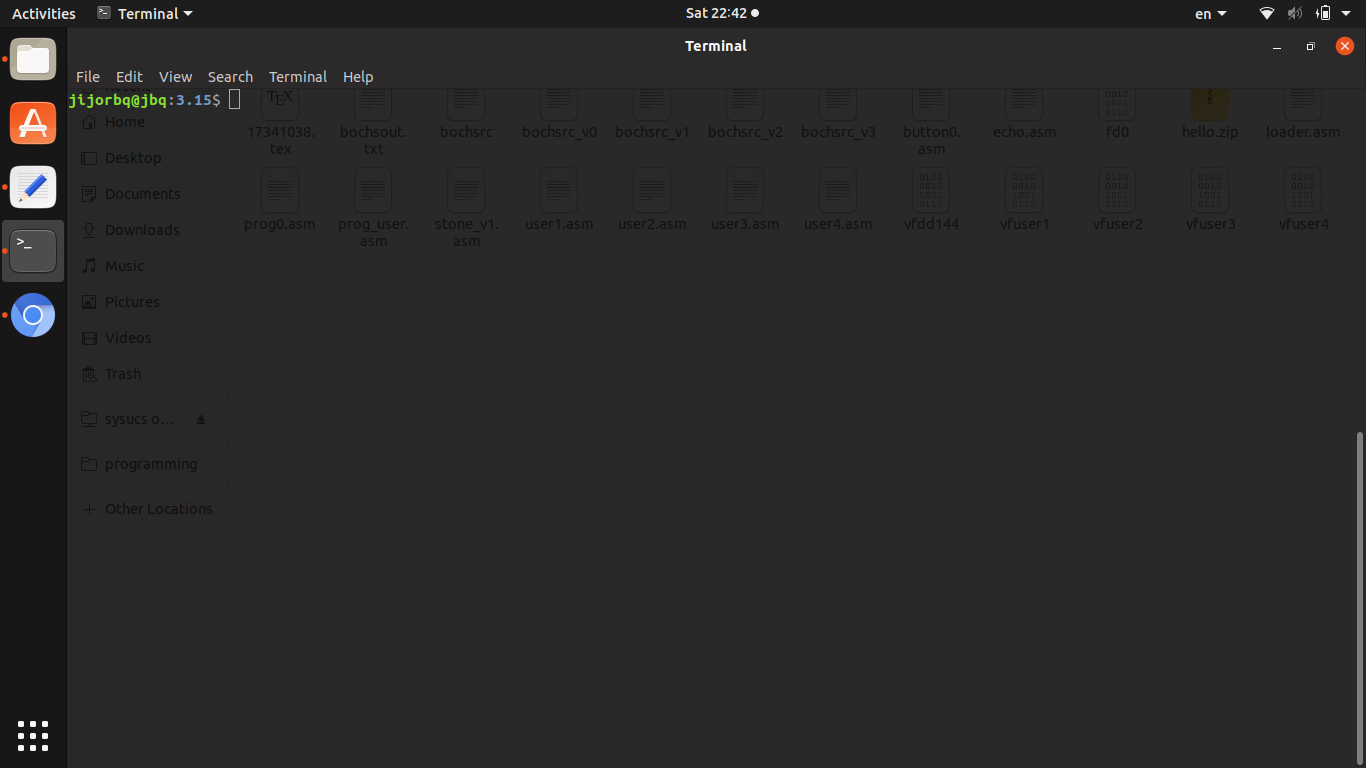
\includegraphics[width=7cm]{Screenshot from 2019-03-23 22-42-23.png}
		\quad
	}
\end{figure}
	\begin{figure}[htbp]{
		\centering
		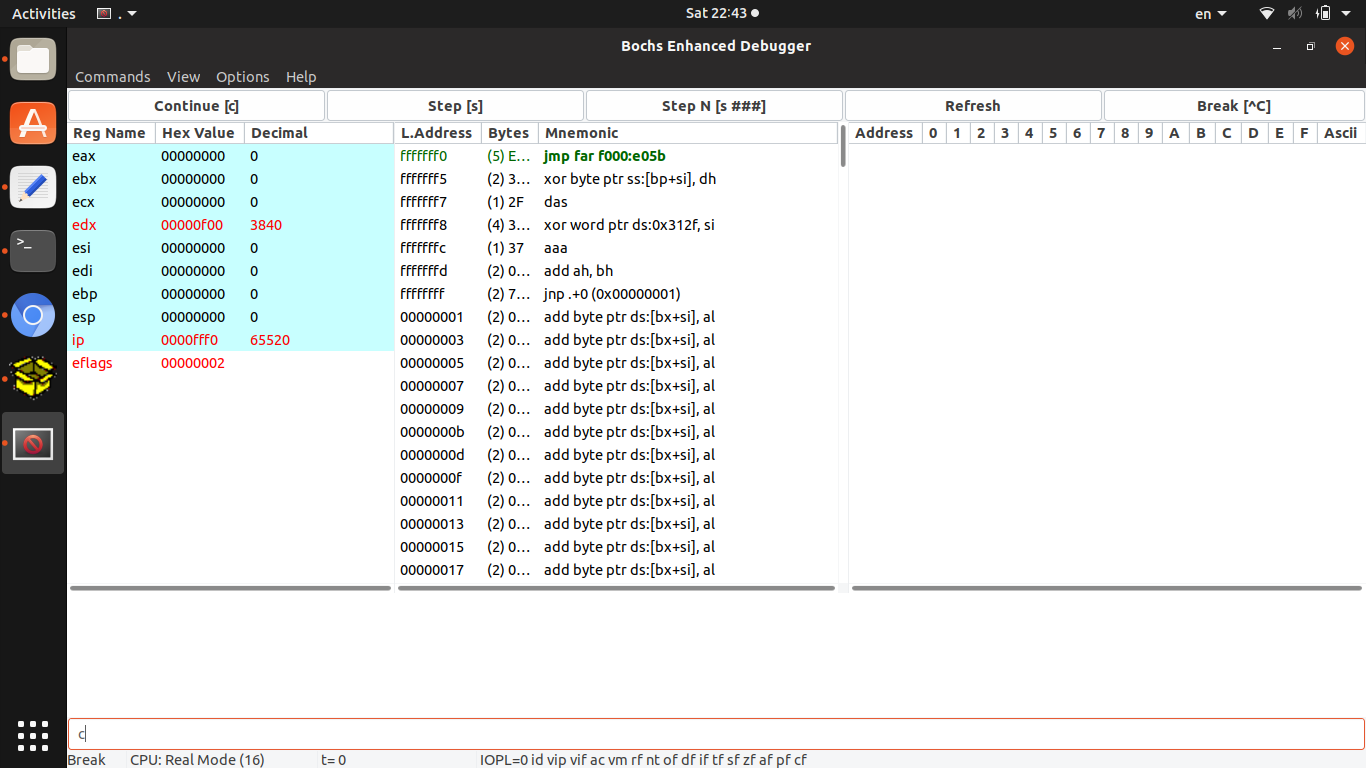
\includegraphics[width=7cm]{Screenshot from 2019-03-23 22-43-02.png}
	}
\end{figure}

启动之后:

\begin{figure}[htbp]{
	\centering
		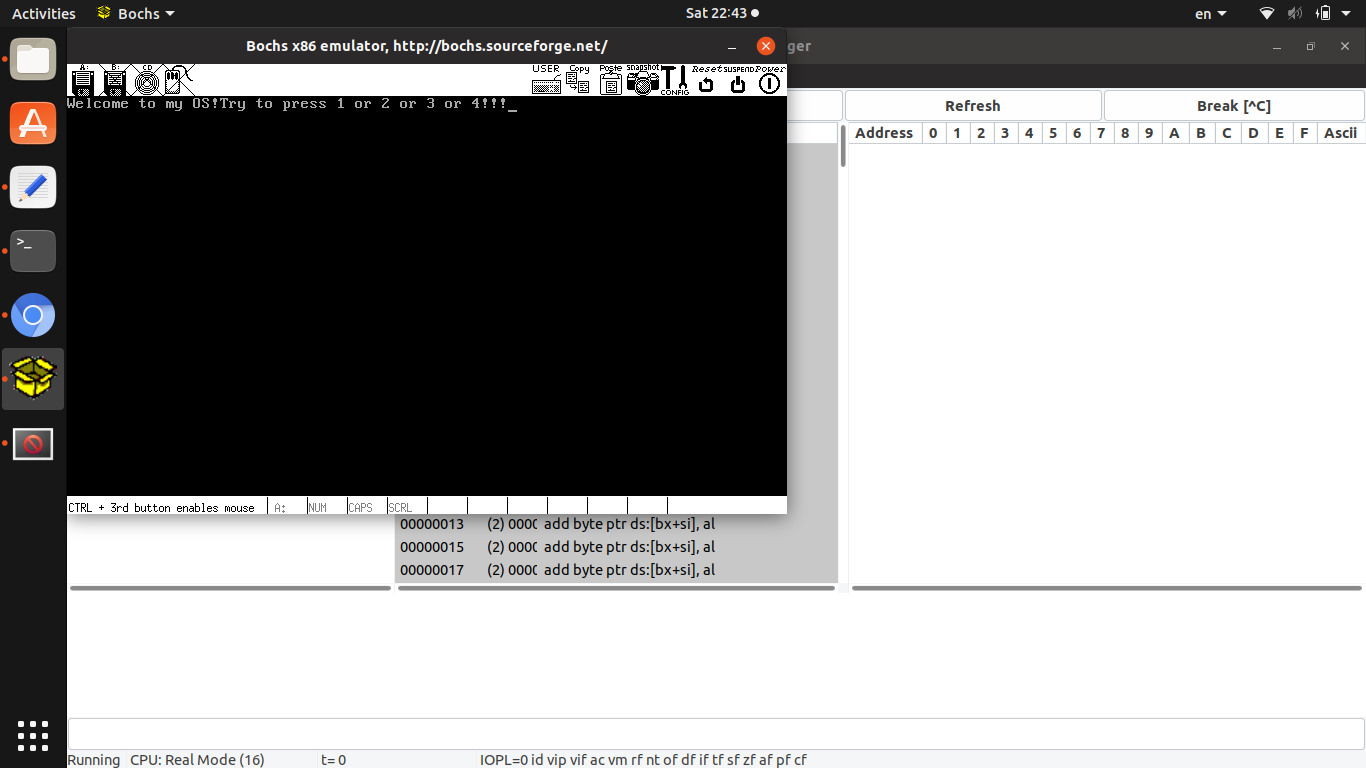
\includegraphics[width=7cm]{Screenshot from 2019-03-23 22-43-10.png}
	\quad
}
\end{figure}

\begin{figure}[htbp]{
	\centering
		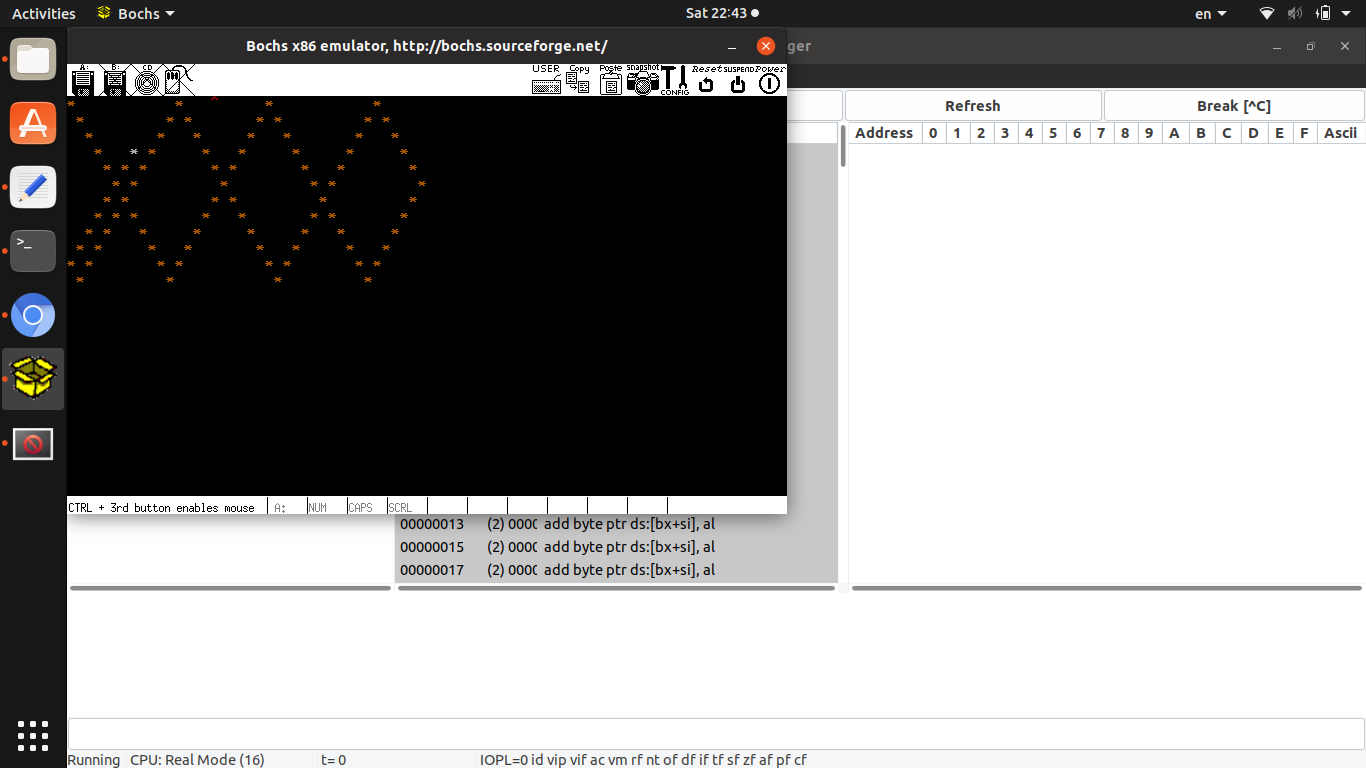
\includegraphics[width=7cm]{Screenshot from 2019-03-23 22-43-19.png}
	\quad
}
\end{figure}
\begin{figure}[htbp]{
	\centering
		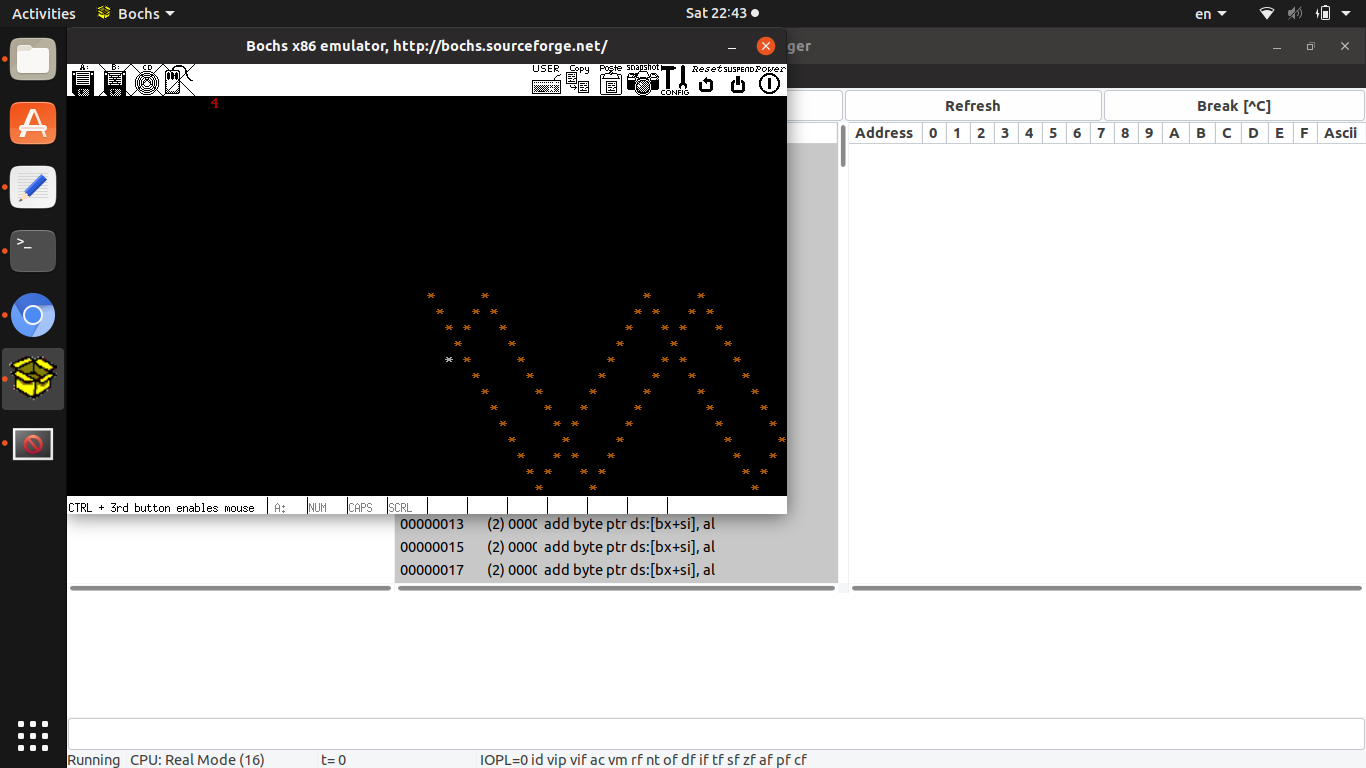
\includegraphics[width=7cm]{Screenshot from 2019-03-23 22-43-33.png}
		\quad
}
\end{figure}
\begin{figure}[htbp]{
	\centering
		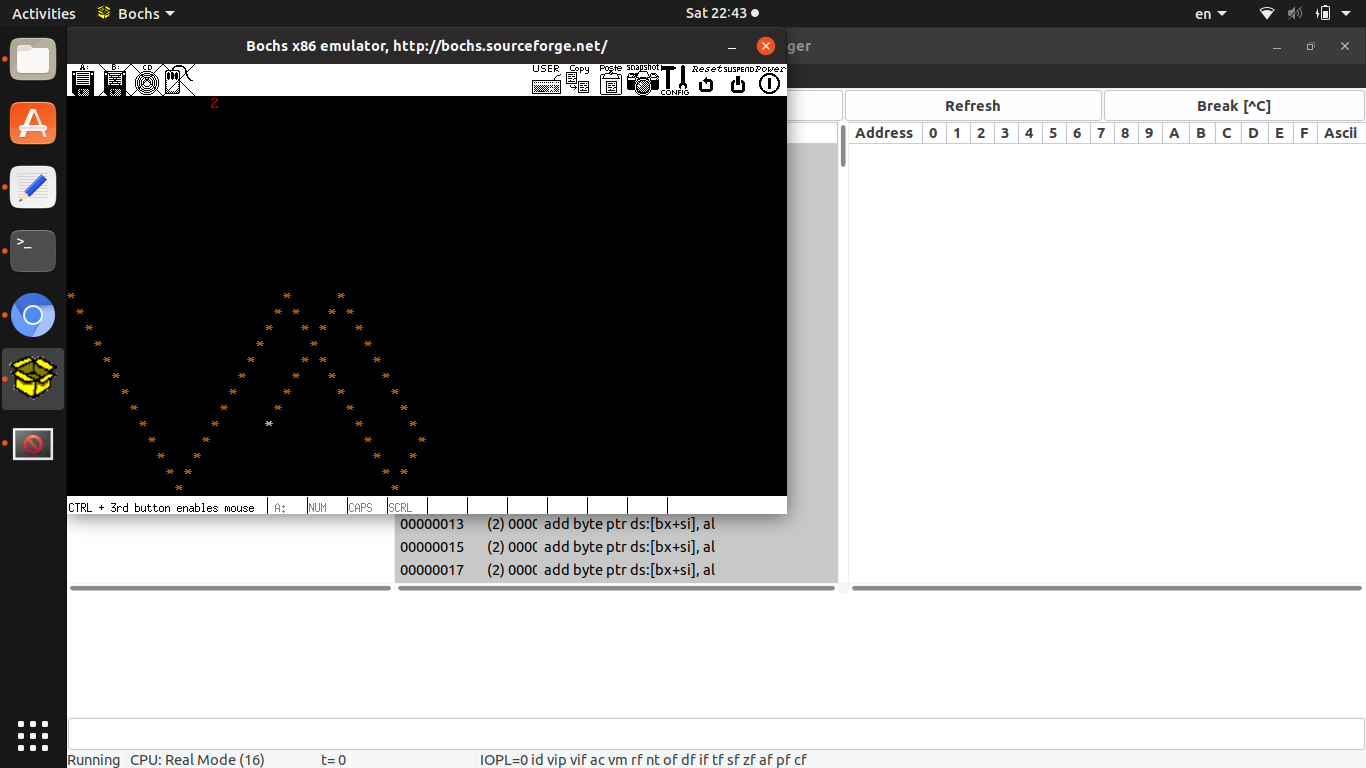
\includegraphics[width=7cm]{Screenshot from 2019-03-23 22-43-41.png}
		\quad
	}
\end{figure}
\subsection{疑难问题解决}
	
	\begin{itemize}
		\item 代码版本管理不善,一些bugs被反反复复的在各个不同的文件夹中的同一份代码里debug,效率及其底下
	
		
		\item 对中断功能的了解不够,带着误解去使用这些中断的功能导致自己浪费大量的时间。
		
		\item 用户程序的起始物理地址没有很好的在各个用户程序中妥善修改,导致用户程序不能被正确执行。
	\end{itemize}


\section{实验总结}
本次实验算是从引导扇区向广阔的内存空间跳跃的一个非常重要的一步。
之前经常听到主引导记录这个名词,但是对于它的理解并不深,只知道它在系统加载的时候很重要。
现在我想自己写一个操作系统,第一步就是它了。
这次实验难度比较大的地方,体现在编码难度开始增加,操作系统“大”而“繁”的标签开始显现出来,对代码实现,工程思维水平开始有一定的挑战。
代码管理不善,命名不统一不规范所带来的弊端,开始超过以前它所带给我的一些方便了。所以从下个实验开始,科学严谨的编程习惯就是必不可少的了。

\section{参考文献}

\bibliographystyle{plain}
\bibliography{ref}

\clearpage


\end{document}
